%!TEX root = main-cav.tex

\section{Decision procedure for the non-zero output problem}\label{sec:dec-snt}
%
We prove our main result, Theorem~\ref{thm:correctness}, by presenting a decision procedure for the non-zero output problem of SNTs. We fix an SNT $\Ss = (Q,X,Y,\delta,q_0,O)$ such that $X=\{ x_1,\dots, x_k\}$ and $Y = \{y_1,\dots,y_l\}$. 
%Due to space constraint, we only present a simplified version where the transition guards are constant-free and leave the procedure for the general case in the full version.
We first define summaries of the computations of $\Ss$ on paths and cycles in Section~\ref{sec-sum}, then present a decision procedure for the case that the transition graph of $\Ss$ is a \emph{generalized lasso} in Section~\ref{sec-glasso}. The transition graph of $\Ss$ is said to be a generalized lasso if it comprises a handle $H=q_0 \xrightarrow{(g_1,\eta_1)} q_1 \dots q_{m-1} \xrightarrow{(g_m,\eta_m)} q_{m}$ and a collection of simple cycles $C_1,\dots,C_n$ such that $q_m$ is the unique state shared by each pair of distinct cycles from $\{C_1,\dots,C_n\}$. We extend the procedure to SNTs whose transition graphs are not necessarily generalized lassos in Section~\ref{sec-gflat}. 


\begin{theorem}\label{thm:correctness}
The non-zero output problem of SNTs can be decided in time exponential in the number of data variables and the maximum number of simple cycles in an SCC of transition graphs.
\end{theorem}
%\vspace{-2mm}

\begin{corollary}\label{cor:snt-dec-proc}
The commutativity problem of  reducer programs can be decided in time exponential in the number of data variables, and doubly exponential in the number of branching statements of reducer programs. 
%On the other hand, the commutativity problem of reducer programs can be decided in time exponential over the number of control variables and the number of data variables, but .
\end{corollary}

\begin{remark}
Though the decision procedure for the commutativity problem of reducer programs has a complexity exponential in the number of data variables, and doubly exponential in the number of branching statements, we believe that the decision procedure could still be implemented to automatically analyze the programs in practice, in which these numbers are usually small. 
\end{remark}

%!TEX root = main-cav.tex

%\vspace{-4mm}
\subsection{Summarization of the computations on paths and cycles}\label{sec-sum}
%\vspace{-1mm}

Suppose $P=p_0 \xrightarrow{(g_1,\eta_1)} p_1 \dots p_{n-1} \xrightarrow{(g_n,\eta_n)} p_{n}$ is a path of $\Ss$. We assume that the initial values of the control and data variables are represented by a symbolic valuation $\sval$ over $X \cup Y$ such that for each pair of variables $x_i, x_j \in X$, $\sval(x_j)=\sval(x_j)$ iff $x_i \sim_{p_0} x_j$. When $P$ is traversed in a run of $\Ss$ over a data word $w$,  the data value in a position of $w$ may have to be (un)equal to the initial value of some control variable or some other data value in $w$ that have been met before (enforced by the guards and assignments in $P$). Let $\sim_P$ denote the equivalence relation on $[n+k]$ induced by $P$ defined as follows: 
\begin{itemize}
\item For each $i, j \in [k]$, $i \sim_P j$ iff $x_i \sim_{p_0} x_j$.
%
\item For each $i, j \in [n]$, $k+i \sim_P k+j$ iff the guards and assignments on $P$ enforce that the data value in the $i$-th position of $w$ must be equal to that in the $j$-th position of $w$.
%
\item For each $i \in [k]$ and $j \in [n]$, $i \sim_P k+j$ iff the guards and assignments on $P$ enforce that the data value in the $j$-th position of $w$ must be equal to the initial value of $x_i$. 
\end{itemize}
Assuming that there are $r^{\circled{P}}$ ``\emph{fresh}'' equivalence classes of $\sim$, that is, equivalence classes $J$ of $\sim_P$ such that $J \cap [k] = \emptyset$ (intuitively, the data value represented by $J$ is not enforced to be equivalent to the initial values of control variables). 
We use the variables $\vard^{\circled{P}}_1,\vard^{\circled{P}}_2,\dots, \vard^{\circled{P}}_{r^{\circled{P}}}$ to denote the data values corresponding to these ``fresh'' equivalence classes, one for each such equivalence class. Note here we use the superscript ${\circled{P}}$ to denote the fact that $r^{\circled{P}}$ (resp. $\vard^{\circled{P}}_1$, $\dots$) is associated with the path $P$. In addition, we assume that there are $s^{\overline{p_0}}$ equivalence classes of $\sim_P$ on $[k]$, that is, equivalence classes $J$ of $\sim_P$ on $[n+k]$ such that $J \cap [k] \neq \emptyset$. Suppose $J_1,\dots, J_{s^{\circled{p_0}}}$ is an enumeration of these equivalence classes of $\sim_P$. Let $\pi^{\circled{p_0}}: [s^{\circled{p_0}}] \rightarrow [k]$ such that $\pi^{\circled{p_0}}(j) = \min(J_j \cap [k])$ for each $j \in [s^{\circled{p_0}}]$. Intuitively, $\pi^{\circled{p_0}}$ chooses a representative control variable for each equivalence class. Note that $\pi^{\circled{p_0}}$ is an injective function, moreover, $s^{\circled{p_0}}$ and $\pi^{\circled{p_0}}$ are completely determined by $\sim_{p_0}$.
%Moreover, let $\varpi^{\circled{p_0}}: [k] \rightarrow [k]$ such that $\varpi^{\circled{p_0}}(j) = \min(\{j' \in [k] \mid j \sim_{p_0} j'\})$.

\begin{example}
Let $\Ss$ be an SNT where $X=\{x\}$, $Y=\{y\}$, and $P = p_0 \xrightarrow{(g_1,\eta_1)} p_1 \xrightarrow{(g_2,\eta_2)} p_2  \xrightarrow{(g_3,\eta_3)} p_3$ be a path of $\Ss$ such that $(g_1,\eta_1) = (\cur = x, y:= \cur)$, $(g_2,\eta_2)= (\ltrue, (x:=\cur, y:=y+\cur))$, $(g_3,\eta_3)= (\cur=x, y:=y+\cur)$. Then $k=1$, $n=3$. The guards and assignments enforce that the data value in position $1$ is equal to the initial value of $x$, which implies that $1 \sim_P 1+1$, i.e. $1 \sim_P 2$, in addition, the data value in position $2$ is equal to that in position $3$, which implies that $1+2 \sim_P 1+3$, i.e. $3 \sim_P 4$. Therefore, the equivalence relation $\sim_P$ has two equivalence classes, $\{1,2\}$ and $\{3,4\}$, of which $\{3,4\}$ is the fresh equivalence class. We conclude that $r^{\circled{P}}=1$ and $\vard^{\circled{P}}_1$ is used to denote the data value corresponding to this fresh equivalence class.
\end{example}

\hide{
Suppose $P=p_0 \xrightarrow{(g_1,\eta_1)} p_1 \dots p_{n-1} \xrightarrow{(g_n,\eta_n)} p_{n}$ is a path of $\Ss$. We assume that the initial values of the control and data variables are represented by a symbolic valuation $\sval$ over $X \cup Y$. 
We use the variables $\vard^{\circled{P}}_1,\vard^{\circled{P}}_2,\dots, \vard^{\circled{P}}_{r^{\circled{P}}}$ to denote the data values introduced while traversing $P$. Notice that according to Proposition~\ref{prop-snt-distinct-value}, one can choose different values for different positions of $P$. Therefore, for each position of $P$, a fresh variable is introduced to represent the data value in that position. Thus we have $r^{\circled{P}}=n$. Here we use the superscript ${\circled{P}}$ to denote the fact that $r^{\circled{P}}$ (resp. $\vard^{\circled{P}}_1$, $\dots$) is associated with the path $P$. 
}


%for variables $\vard^{\circled{P}}_i,\vard^{\circled{P}}_j$ for $1\leq i< j \leq r^{\circled{P}}$ according to our definition of guards; they will never force the values of $\vard^{\circled{P}}_i$ and $\vard^{\circled{P}}_j$ to be equivalent.


%When $P$ is traversed in a run of $\Ss$ over a data word $w$,  the data value in a position of $w$ may have to be (un)equal to the initial value of some control variable or some other data value in $w$ that have been met before (enforced by the guards and assignments in $P$). Let $\sim$ denote the equivalence relation on $[n]$ induced by $P$ such that $i \sim j$ iff the guards and assignments on $P$ enforce that the data value in the $i$-th position of $w$ must be equal to that in the $j$-th position of $w$. Assuming that there are $r^{\circled{P}}$ ``\emph{fresh}'' equivalence classes of $\sim$, that is, equivalence classes whose values are not enforced to be equivalent to the initial values of control variables. 
%We use the variables $\vard^{\circled{P}}_1,\vard^{\circled{P}}_2,\dots, \vard^{\circled{P}}_{r^{\circled{P}}}$ to denote the data values corresponding to these ``fresh'' equivalence classes, one for each such equivalence class. Note here we use the superscript ${\circled{P}}$ to denote the fact that $r^{\circled{P}}$ (resp. $\vard^{\circled{P}}_1$, $\dots$) is associated with the path $P$.

\begin{proposition}\label{prop-sum-path}
Suppose that $P$ is a path starting form $p_0$ and the initial values of $X \cup Y$ are represented by a symbolic valuation $\initval$ such that such that for each pair of variables $x_i, x_j \in X$, $\sval(x_j)=\sval(x_j)$ iff $x_i \sim_{p_0} x_j$. Then the values of $X \cup Y$ after traversing the path $P$ are specified by a symbolic valuation $\sumf^{(P,\initval)}$ satisfying the following conditions.
\begin{itemize}
\item The set of indices of $X$, i.e., $[k]$, is partitioned into $I^{\circled{P}}_{pe}$ and $I^{\circled{P}}_{tr}$, the indices of \emph{persistent} and \emph{transient} control variables, respectively. A control variable is persistent if it stores the initial value of some control variable after traversing $P$, otherwise, it is transient.
\item For each $x_j\in X$ such that $j \in I^{\circled{P}}_{pe}$, $\sumf^{(P,\initval)}(x_j)=\sval(x_{\pi^{\circled{p_0}}(\pi^{\circled{P}}_{pe}(j))})$, where $\pi^{\circled{P}}_{pe}: I^{\circled{P}}_{pe} \rightarrow [s^{\circled{p_0}}]$ is a mapping from the index of a persistent control variable $x_j$ to the index of the equivalence class such that the initial value of control variables corresponding to this equivalence class is assigned to $x_j$ after traversing $P$.
%
\item  For each $x_j\in X$ such that $j\in I^{\circled{P}}_{tr}$,
$\sumf^{(P,\initval)}(x_j)=\vard^{\circled{P}}_{\pi^{\circled{P}}_{tr}(j)}$, where $\pi^{\circled{P}}_{tr}: I^{\circled{P}}_{tr} \rightarrow [r^{\circled{P}}]$ is a mapping from the index of a transient control variable to the index of the data value assigned to it.
% 
\item For each $y_j \in Y$, 
\[
 \sumf^{(P,\initval)}(y_j)  =
 \cste^{\circled{P}}_{j} + 
 \cstl^{\circled{P}}_j \initval(y_j)  + 
  \sum\limits_{j'\in [s^{\circled{p_0}}]} \csta^{\circled{P}}_{j,j'}\initval(x_{\pi^{\circled{p_0}}(j')}) +
  \sum\limits_{j''\in [r^{\circled{P}}]}\cstb^{\circled{P}}_{j,j''} \vard^{\circled{P}}_{j''},
\]  
%%%%%%%%%%%%%%%%%%%%%%%%%%%%%%%%%%%%%%%%%%%
%%%%%%%%%%%%%%%%%%%%%%%%%%%%%%%%%%%%%%%%%%%
\hide{
\item For each $y_j \in Y$, 
\[
\small
\begin{array}{l}
\smallskip
\sumf^{(P,\initval)}(y_j)  = \\
\hspace{2mm} \cste^{\circled{P}}_{j} + \cstl^{\circled{P}}_j \initval(y_j)  + \csta^{\circled{P}}_{j,1} \initval(x_1) + \dots + \csta^{\circled{P}}_{j,k} \initval(x_k) +  \cstb^{\circled{P}}_{j,1} \vard^{\circled{P}}_1 +\dots + \cstb^{\circled{P}}_{j,r^{\circled{P}}} \vard^{\circled{P}}_{r^{\circled{P}}},
\end{array}
\]} 
%%%%%%%%%%%%%%%%%%%%%%%%%%%%%%%%%%%%%%%%%%%
%%%%%%%%%%%%%%%%%%%%%%%%%%%%%%%%%%%%%%%%%%%
where $\cste^{\circled{P}}_j,\cstl^{\circled{P}}_j, \csta^{\circled{P}}_{j,1},\dots,\csta^{\circled{P}}_{j, s^{\circled{p_0}}}, \cstb^{\circled{P}}_{j,1},\dots,\cstb^{\circled{P}}_{j,r^{\circled{P}}}$ are integer constants such that $\cstl^{\circled{P}}_{j} \in \{0,1\}$ (as a result of the ``independently evolving and copyless'' constraint).  It can happen that $\cstl^{\circled{P}}_j =0$,  which means that $\initval(y_j)$ is irrelevant to $\sumf^{(P,\initval)}(y_j)$. Similarly for $\csta^{\circled{P}}_{j,1}=0$, and so on.
\end{itemize}
\end{proposition}
In Proposition~\ref{prop-sum-path}, the sets $I^{\circled{P}}_{pe}$ and $I^{\circled{P}}_{tr}$, the mapping $\pi^{\circled{P}}_{pe}$ and $\pi^{\circled{P}}_{tr}$, and the constants $\cste^{\circled{P}}_j,\cstl^{\circled{P}}_j, \dots, \cstb^{\circled{P}}_{j,r^{\circled{P}}}$ only depend on $P$ and are independent of $\initval$. In addition, they can be computed in polynomial time from (the transitions in) $P$.
%Due to the uniquely-valued constraint of normalized SNTs, $\pi^{\circled{P}}$ is injective, 
We define $(\pi^{\circled{P}}_{pe})^{-1}$ as the inverse function of $\pi^{\circled{P}}_{pe}$, that is, for each $j' \in \rng(\pi^{\circled{P}}_{pe})$, $(\pi^{\circled{P}}_{pe})^{-1}(j')=\{j \in I^{\circled{P}}_{pe}  \mid \pi^{\circled{P}}(j)= j'\}$. Similarly for $(\pi^{\circled{P}}_{tr})^{-1}$.

As a corollary of Proposition~\ref{prop-sum-path}, the following result demonstrates how to summarize the computations of $\Ss$ on the composition of two paths.

\begin{corollary}\label{cor-comp-two-paths}
Suppose that $P_1$ and $P_2$ are two paths in $\Ss$ such that the last state of $P_1$ is the same as the first state of $P_2$. Moreover, let $\sumf^{(P_1, \initval)}$ (resp. $\sumf^{(P_2, \initval)}$) be the symbolic valuation summarizing the computation of $\Ss$ on $P_1$ (resp. $P_2$). Then the symbolic valuation summarizing the computation of $\Ss$ on $P_1 P_2$ is $\sumf^{(P_2,\ \sumf^{(P_1,\initval)})}$.
\end{corollary}

Let the first state of $P_1$ and $P_2$ be $p_{1,0}$ and $p_{2,0}$ respectively. In order to get a better understanding of the relation between $\sumf^{(P_2,\ \sumf^{(P_1,\initval)})}$ and $(\sumf^{(P_1, \initval)},\sumf^{(P_2, \initval)})$, in the following, for each $y_j \in Y$, we obtain a more explicit form of the expression $\sumf^{(P_2,\ \sumf^{(P_1,\initval)})}(y_j)$, by unfolding therein the expression $\sumf^{(P_1,\initval)}$,\\
%
\medskip
\resizebox{\hsize}{!}{
	$\begin{array}{rl}
	\medskip
	\sumf^{(P_2,\ \sumf^{(P_1,\initval)})}(y_j) = & 
	\left(\cste^{\circled{P_2}}_{j}+
	\cstl^{\circled{P_2}}_{j} \cste^{\circled{P_1}}_{j}\right)+ \left(\cstl^{\circled{P_2}}_{j} \cstl^{\circled{P_1}}_{j} \right) \initval(y_j)\ +\\
	\medskip
	& \sum \limits_{j' \in \rng(\pi^{\circled{P_1}}_{pe})} 
	\left(\cstl^{\circled{P_2}}_{j} \csta^{\circled{P_1}}_{j,j'} + \sum \limits_{j'' \in (\pi^{\circled{P_1}}_{pe})^{-1}(j')\ \cap\ \rng(\pi^{\circled{p_{2,0}}})}  \csta^{\circled{P_2}}_{j,(\pi^{\circled{p_{2,0}}})^{-1}(j'')} \right) \initval(x_{\pi^{\circled{p_{1,0}}}(j')})\ + \\
	\medskip
	& 
	\sum \limits_{j' \in  [s^{\circled{p_{1,0}}}] \setminus \rng(\pi^{\circled{P_1}}_{pe}) } 
	\left(\cstl^{\circled{P_2}}_{j} \csta^{\circled{P_1}}_{j,j'} \right) \initval(x_{\pi^{\circled{p_{1,0}}}(j')})\ +\\
	\medskip
	& \sum \limits_{j' \in \rng(\pi^{\circled{P_1}}_{tr})} \left(\cstl^{\circled{P_2}}_{j} \cstb^{\circled{P_1}}_{j,j'} + \sum \limits_{j'' \in (\pi^{\circled{P_1}}_{tr})^{-1}(j') \cap \rng(\pi^{\circled{p_{2,0}}})} \csta^{\circled{P_2}}_{j, (\pi^{\circled{p_{2,0}}})^{-1}(j'')} \right) \vard^{\circled{P_1}}_{j'}\ +
	 \\
	%
	& 
	\sum \limits_{j' \in [r^{\circled{P_1}}]\setminus \rng(\pi^{\circled{P_1}}_{tr})} \left( \cstl^{\circled{P_2}}_{j} \cstb^{\circled{P_1}}_{j,j'} \right) \vard^{\circled{P_1}}_{j'} +
	
	\sum \limits_{j'\in[r^{\circled{P_2}}]} \cstb^{\circled{P_2}}_{j,j'} \vard^{\circled{P_2}}_{j'}.
	\end{array}$
}\medskip\\
In the equation, $j' \in  \rng(\pi^{\circled{P_1}}_{pe})$ implies that for each $j'' \in  (\pi^{\circled{P_1}}_{pe})^{-1}(j')$,  $x_{j''}$ stores the initial value of $x_{\pi^{\circled{p_{1,0}}}(j')}$ after traversing $P_1$, which means that the initial value of $x_{j''}$ for each $j'' \in  (\pi^{\circled{P_1}}_{pe})^{-1}(j')$ before traversing $P_2$ is $\initval(x_{\pi^{\circled{p_{1,0}}}(j')})$, and some of $x_{j''}$ for $j'' \in  (\pi^{\circled{P_1}}_{pe})^{-1}(j')$ are chosen as the representatives of the equivalence classes of $\sim_{p_{2,0}}$ (in this case, $j''$ is in the range of $\pi^{\circled{p_{2,0}}}$), therefore we have the item $\left( \sum \limits_{j'' \in (\pi^{\circled{P_1}}_{pe})^{-1}(j')\ \cap\ \rng(\pi^{\circled{p_{2,0}}})}  \csta^{\circled{P_2}}_{j,(\pi^{\circled{p_{2,0}}})^{-1}(j'')} \right) \initval(x_{\pi^{\circled{p_{1,0}}}(j')})$. When $j' \in \rng(\pi^{\circled{P_1}}_{tr})$, the initial value of $x_{j''}$ for each $j'' \in (\pi^{\circled{P_1}}_{tr})^{-1}(j')$ before traversing $P_2$ is $\vard^{\circled{P_1}}_{j'}$, and some of $x_{j''}$ for $j'' \in (\pi^{\circled{P_1}}_{tr})^{-1}(j')$ are chosen as the representatives of equivalence classes of $\sim_{p_{2,0}}$, therefore we have the item $\left(\sum \limits_{j'' \in (\pi^{\circled{P_1}}_{tr})^{-1}(j') \cap \rng(\pi^{\circled{p_{2,0}}})} \csta^{\circled{P_2}}_{j, (\pi^{\circled{p_{2,0}}})^{-1}(j'')} \right)\ \vard^{\circled{P_1}}_{j'}$.
For all $j'\in [s^{\circled{p_{1,0}}}] =\rng(\pi^{\circled{P_1}}_{pe}) \cup ([s^{\circled{p_{1,0}}}] \setminus \rng(\pi^{\circled{P_1}}_{pe}))$, we have the item $(\cstl^{\circled{P_2}}_{j} \csta^{\circled{P_1}}_{j,j'}) \initval(x_{\pi^{\circled{p_{1,0}}}(j')})$, i.e. the coefficient of $\initval(x_{\pi^{\circled{p_{1,0}}}(j')})$ in $\sumf^{(P_1, \initval)}$ multiplied by $\cstl^{\circled{P_2}}_{j}$. Moreover, for all $j'\in [r^{\circled{P_1}}] = \rng(\pi^{\circled{P_1}}_{tr}) \cup ([r^{\circled{P_1}}] \setminus \rng(\pi^{\circled{P_1}}_{tr}))$, we have 
the item $( \cstl^{\circled{P_2}}_{j} \cstb^{\circled{P_1}}_{j,j'}) \vard^{\circled{P_1}}_{j'}$, i.e. the coefficient of $\vard^{\circled{P_1}}_{j'}$ in $\sumf^{(P_1, \initval)}$ multiplied by $\cstl^{\circled{P_2}}_{j}$.

In the following, by utilizing Proposition~\ref{prop-sum-path} and Corollary~\ref{cor-comp-two-paths}, for each path $C^{\ell}$ ($\ell \ge 1$) which is obtained by iterating a simple cycle $C = (q, g, \eta, q)$ for $\ell$ times, we illustrate how $\sumf^{(C^\ell,\initval)}$ is related to $\sumf^{(C, \initval)}$ and $\ell$. For convenience, we call $\ell$ a \emph{cycle counter variable}. It is easy to observe that both $I^{\circled{C}}_{pe}$ and $I^{\circled{C}}_{tr}$ are the union of the equivalence classes of $\sim_{q}$. From the ``Monotone'' constraint, we know that for each $x \in \dom(\eta)$, it holds that $\eta(x)=\cur$. Therefore, if $j \in I^{\circled{C}}_{pe}$, then $x_j$ still stores the initial value of $x_j$ after traversing $C$. 
%
This implies that for each $j' \in \rng(\pi^{\circled{C}}_{pe})$, let $\pi^{\circled{q}}(j')=j$, then $\pi^{\circled{C}}_{pe}(j)=j'$.  Therefore, for each $j' \in \rng(\pi^{\circled{C}}_{pe})$, the value of $x_{\pi^{\circled{q}}(j')}$ is unchanged after traversing $C$.
\begin{proposition}\label{prop-sum-cycle}
Suppose that $C$ is a simple cycle (i.e. a self-loop) and $P=C^{\ell}$ such that $\ell \ge 2$. Then the symbolic valuation $\sumf^{(C^\ell,\initval)}$ to summarize the computation of $\Ss$ on $P$ is as follows:  
%\begin{itemize}
%\item If $r^{\circled{C}}=1$, then

\noindent
\medskip
\resizebox{0.95\hsize}{!}{
$
\begin{array}{l c l}
\sumf^{(C^\ell,\initval)}(y_j)  &= & 
\left(1 + \cstl^{\circled{C}}_{j} + \dots +(\cstl^{\circled{C}}_{j})^{\ell - 1} \right)\cste^{\circled{C}}_{j} + (\cstl^{\circled{C}}_{j})^\ell \initval(y_j)\ + \\
\smallskip
%
&& \sum \limits_{j' \in \rng(\pi^{\circled{C}}_{pe}) } \left(1+\cstl^{\circled{C}}_{j} + \dots +(\cstl^{\circled{C}}_{j})^{\ell - 1} \right) \csta^{\circled{C}}_{j,j'}\initval(x_{\pi^{\circled{q}}(j')}) \ + \\
& &  \sum \limits_{j' \in [s^{\circled{q}}] \setminus \rng(\pi^{\circled{C}}_{pe}) }  (\cstl^{\circled{C}}_{j})^{\ell - 1} \csta^{\circled{C}}_{j,j'} \initval(x_{\pi^{\circled{q}}(j')})\ +  \\
\smallskip
%
&&  \sum \limits_{j' \in \rng(\pi^{\circled{C}}_{tr})} \sum \limits_{s\in[\ell -1]}
\left(\cstl^{\circled{C}}_{j}\cstb^{\circled{C}}_{j,j'}+ \sum \limits_{j'' \in (\pi^{\circled{C}}_{tr})^{-1}(j') \cap \rng(\pi^{\circled{q}})} \csta^{\circled{C}}_{j, (\pi^{\circled{q}})^{-1}(j'')}  \right)
(\cstl^{\circled{C}}_{j})^{\ell-s-1}
\vard^{\circled{C , s}}_{j'}\ +\\
\smallskip
%
&& \sum \limits_{j' \in [r^{\circled{C}}] \setminus \rng(\pi^{\circled{C}}_{tr})}\sum \limits_{s\in[\ell -1]} \left((\cstl^{\circled{C}}_{j})^{\ell - s} \cstb^{\circled{C}}_{j,j'} \right) \vard^{\circled{C , s}}_{j'} + 
\sum \limits_{j' \in [r^{\circled{C}}] }  
 \cstb^{\circled{C}}_{j, j'} \vard^{\circled{C , \ell}}_{j'},
\end{array} 
$
}
\medskip\\
where the variables $\vard^{\circled{C , s}}_{1}$ for $s\in [\ell]$
 represent the data values introduced when traversing $C$ for the $s$-th time. 
%
%%%%%%%%%%%%%%%%%%%%%%%%%%%%%%%%%%%%%%%%%%
\hide{
\item If $r^{\circled{C}}=0$ (no fresh data value introduced when traversing $C$), then
\medskip\\
\resizebox{0.8\hsize}{!}{
$\begin{array}{l c l}
\sumf^{(C^\ell,\initval)}(y_j)  & = & 
\left(1 + \cstl^{\circled{C}}_{j} + \dots +(\cstl^{\circled{C}}_{j})^{\ell - 1} \right)\cste^{\circled{C}}_{j} + (\cstl^{\circled{C}}_{j})^\ell \initval(y_j) + \smallskip\\
%
& & \sum \limits_{j' \in I^{\circled{C}}_{pe}} \left(1+\cstl^{\circled{C}}_{j} + \dots +(\cstl^{\circled{C}}_{j})^{\ell - 1} \right) \csta^{\circled{C}}_{j,j'}\initval(x_{j'}). \\
%+  \sum \limits_{j' \in I^{\circled{C}}_{tr}}  (\cstl^{\circled{C}}_{j})^{\ell - 1} \csta^{\circled{C}}_{j,j'} \initval(x_{j'}). \\
\end{array} 
$}\medskip\\
\end{itemize}
}
\end{proposition}

From Proposition~\ref{prop-sum-cycle} and the fact that $\cstl^{\circled{C}}_{j} \in \{0, 1\}$, we have the following observation.
\begin{itemize}
\item If $\cstl^{\circled{C}}_{j}=0$, then
%
%If $r^{\circled{C}}=1$ and $\cstl^{\circled{C}}_{j}=0$, then
\medskip\\
\resizebox{0.9\hsize}{!}{$
\begin{array}{l c l}
\sumf^{(C^\ell,\initval)}(y_j)  & = & \cste^{\circled{C}}_{j} +  \sum \limits_{j' \in \rng(\pi^{\circled{C}}_{pe})} \csta^{\circled{C}}_{j,j'} \initval(x_{\pi^{\circled{q}}(j')})\ +
\\
&& \sum \limits_{j'  \in \rng(\pi^{\circled{C}}_{tr})} \left(\sum \limits_{j'' \in (\pi^{\circled{C}}_{tr})^{-1}(j') \cap \rng(\pi^{\circled{q}})} \csta^{\circled{C}}_{j, (\pi^{\circled{q}})^{-1}(j'')}  \right) \vard^{\circled{C , \ell  -  1}}_{j'} +  
\sum \limits_{j' \in [r^{\circled{C}}] }  
 \cstb^{\circled{C}}_{j, j'} \vard^{\circled{C , \ell}}_{j'}.
 \end{array}
 $
}
%
\hide{
\item If $r^{\circled{C}}=0$ and $\cstl^{\circled{C}}_{j}=0$, then 
\[
\sumf^{(C^\ell,\initval)}(y_j)   =  \cste^{\circled{C}}_{j} +  \sum \limits_{j' \in I^{\circled{C}}_{pe}} \csta^{\circled{C}}_{j,j'} \initval(x_{j'}).
\]
}
%
\item If $\cstl^{\circled{C}}_{j}=1$, then
%If $r^{\circled{C}}=1$ and $\cstl^{\circled{C}}_{j}=1$, then\medskip\\
\medskip\\
\resizebox{0.95\hsize}{!}{$
\begin{array}{l c l}
\sumf^{(C^\ell,\initval)}(y_j) & = &   \ell \cste^{\circled{C}}_{j}  + \initval(y_j) +   \sum  \limits_{j' \in \rng(\pi^{\circled{C}}_{pe}) } \ell \csta^{\circled{C}}_{j,j'}  \initval(x_{\pi^{\circled{q}}(j')}) + 
\sum \limits_{j' \in [s^{\circled{q}}] \setminus \rng(\pi^{\circled{C}}_{pe})} \csta^{\circled{C}}_{j,j'} \initval(x_{\pi^{\circled{q}}(j')})\ + \\
\smallskip
& & \sum \limits_{j' \in \rng(\pi^{\circled{C}}_{tr})} \sum \limits_{s\in[\ell -1]}
\left(\cstb^{\circled{C}}_{j,j'} + \sum \limits_{j'' \in (\pi^{\circled{C}}_{tr})^{-1}(j') \cap \rng(\pi^{\circled{q}})} \csta^{\circled{C}}_{j, (\pi^{\circled{q}})^{-1}(j'')}  \right) \vard^{\circled{C , s}}_{j'}\ +\\
& &  \sum \limits_{j' \in [r^{\circled{C}}]  \setminus \rng(\pi^{\circled{C}}_{tr}) }\sum \limits_{s\in[\ell -1]} 
\cstb^{\circled{C}}_{j,j'} \vard^{\circled{C , s}}_{j'} + \sum \limits_{j' \in [r^{\circled{C}}] }  
\cstb^{\circled{C}}_{j, j'} \vard^{\circled{C , \ell}}_{j'}.
\end{array}
$
}
%
\hide{
\item If $r^{\circled{C}}=0$ and $\cstl^{\circled{C}}_{j}=1$, then
\[
\sumf^{(C^\ell,\initval)}(y_j)  =    \ell \cste^{\circled{C}}_{j}  + \initval(y_j) +   \sum  \limits_{j' \in I^{\circled{C}}_{pe}} \ell \csta^{\circled{C}}_{j,j'}  \initval(x_{j'}).
\]
}
%
\end{itemize}

%
%From the analysis above, we observe that in $\chi^{\circled{C}}_\ell(y_j)$, 
%\begin{itemize}
%\item the constant coefficient is either $\alpha^{\circled{C}}_{j,0}$, or $\alpha^{\circled{C}}_{j,0} \ell$, 
%
%\item the coefficient of $o_j$ is $0$, or $1$, 
%
%\item for each data value $d^{(0)}_{j'}$, the coefficient of $d^{(0)}_{j'}$ is either $\beta^{\circled{C}}_{j,j'}$, or $0$, or $\beta^{\circled{C}}_{j,j'} \ell$,
%
%\item for each data value $d^{(C , i)}_{j'}$ with $i \ge 1$, the coefficient of $d^{(C , i)}_{j'}$ is either $0$, or $\beta^{\circled{C}}_{j, \pi_C^{-1}(j'+k)}$, or $\beta^{\circled{C}}_{j, \pi_C^{-1}(j'+k)}+\gamma^{\circled{C}}_{j,j'}$, or $\gamma^{\circled{C}}_{j,j'}$.
%\end{itemize}

\begin{example}\label{exmp-sum}
Let $\Ss'_{\sf max}$ be the SNT illustrated in Fig.~\ref{fig-dec-proc-snt-exmp}, which is obtained from $\Ss_{\sf max}$ by replacing  the control variable $\sf max$ with  $x_1$ and introducing the data variables $y_1,y_2, y_3$. Consider the cycle $C_1$ in $\Ss'_{\sf max}$. Then $O(q_2)= a_0 + a_1 x_1 + b_1 y_1 + b_2 y_2 + b_3 y_3 = y_1 - 2y_2 + y_3$. Moreover, $I^{\circled{C_1}}_{pe} = \{1\}$, $I^{\circled{C_1}}_{tr} = \emptyset$, $\pi^{\circled{C_1}}_{pe}(1) = 1$, $\cstl^{\circled{C_1}}_1 = \cstl^{\circled{C_1}}_2 = 1$, and $\cstl^{\circled{C_1}}_3 = 0$. On the other hand, $I^{\circled{C_2}}_{pe} = \emptyset$, $I^{\circled{C_2}}_{tr} = \{1\}$, $\pi^{\circled{C_2}}_{tr}(1) = 1$, and $\cstl^{\circled{C_2}}_1 = \cstl^{\circled{C_2}}_2 = \cstl^{\circled{C_2}}_3  = 1$. Suppose $\ell \ge 2$. Let $ \vard^{\circled{C_1, 1}}_1, \dots, \vard^{\circled{C_1, \ell}}_1$ represent the data values introduced when traversing the path $C^\ell_1$, then
\[
\begin{array}{l c l}
\sumf^{(C^\ell_1, \initval)}(y_1) &= & \initval(y_1) + (4 \ell) \initval(x_1) +\ \ \vard^{\circled{C_1, 1}}_1 + \dots +\ \ \vard^{\circled{C_1, \ell}}_1,\\
%
\sumf^{(C^\ell_1, \initval)}(y_2) &=& \initval(y_2) + (2 \ell) \initval(x_1) + 2 \vard^{\circled{C_1, 1}}_1 + \dots + 2 \vard^{\circled{C_1, \ell}}_1,\\
%
\sumf^{(C^\ell_1, \initval)}(y_3) &=& \hspace{5.5cm} 3 \vard^{\circled{C_1, \ell}}_1.
\end{array}
\] 
On the other hand, let $ \vard^{\circled{C_2, 1}}_1, \dots, \vard^{\circled{C_2, \ell}}_1$ represent the data values introduced when traversing the path $C^\ell_2$, then 
\[
\begin{array}{l c l}
\sumf^{(C^\ell_2, \initval)}(y_1) &= & \initval(y_1) +\ \  \initval(x_1) +4 \vard^{\circled{C_2, 1}}_1 + \dots +4 \vard^{\circled{C_2, \ell-1}}_1 + 3 \vard^{\circled{C_2, \ell}}_1,\\
%
\sumf^{(C^\ell_2, \initval)}(y_2) &=& \initval(y_2) + 3 \initval(x_1) + 5 \vard^{\circled{C_2, 1}}_1 + \dots + 5 \vard^{\circled{C_2, \ell-1}}_1 + 2 \vard^{\circled{C_2, \ell}}_1,\\
%
\sumf^{(C^\ell_2, \initval)}(y_3) &=& \initval(y_3) + 5 \initval(x_1) + 6 \vard^{\circled{C_2, 1}}_1 + \dots + 6 \vard^{\circled{C_2, \ell-1}}_1 + \ \ \vard^{\circled{C_2, \ell}}_1.
\end{array}
\] 

\vspace{-2mm}
\begin{figure}[htbp]
\begin{center}
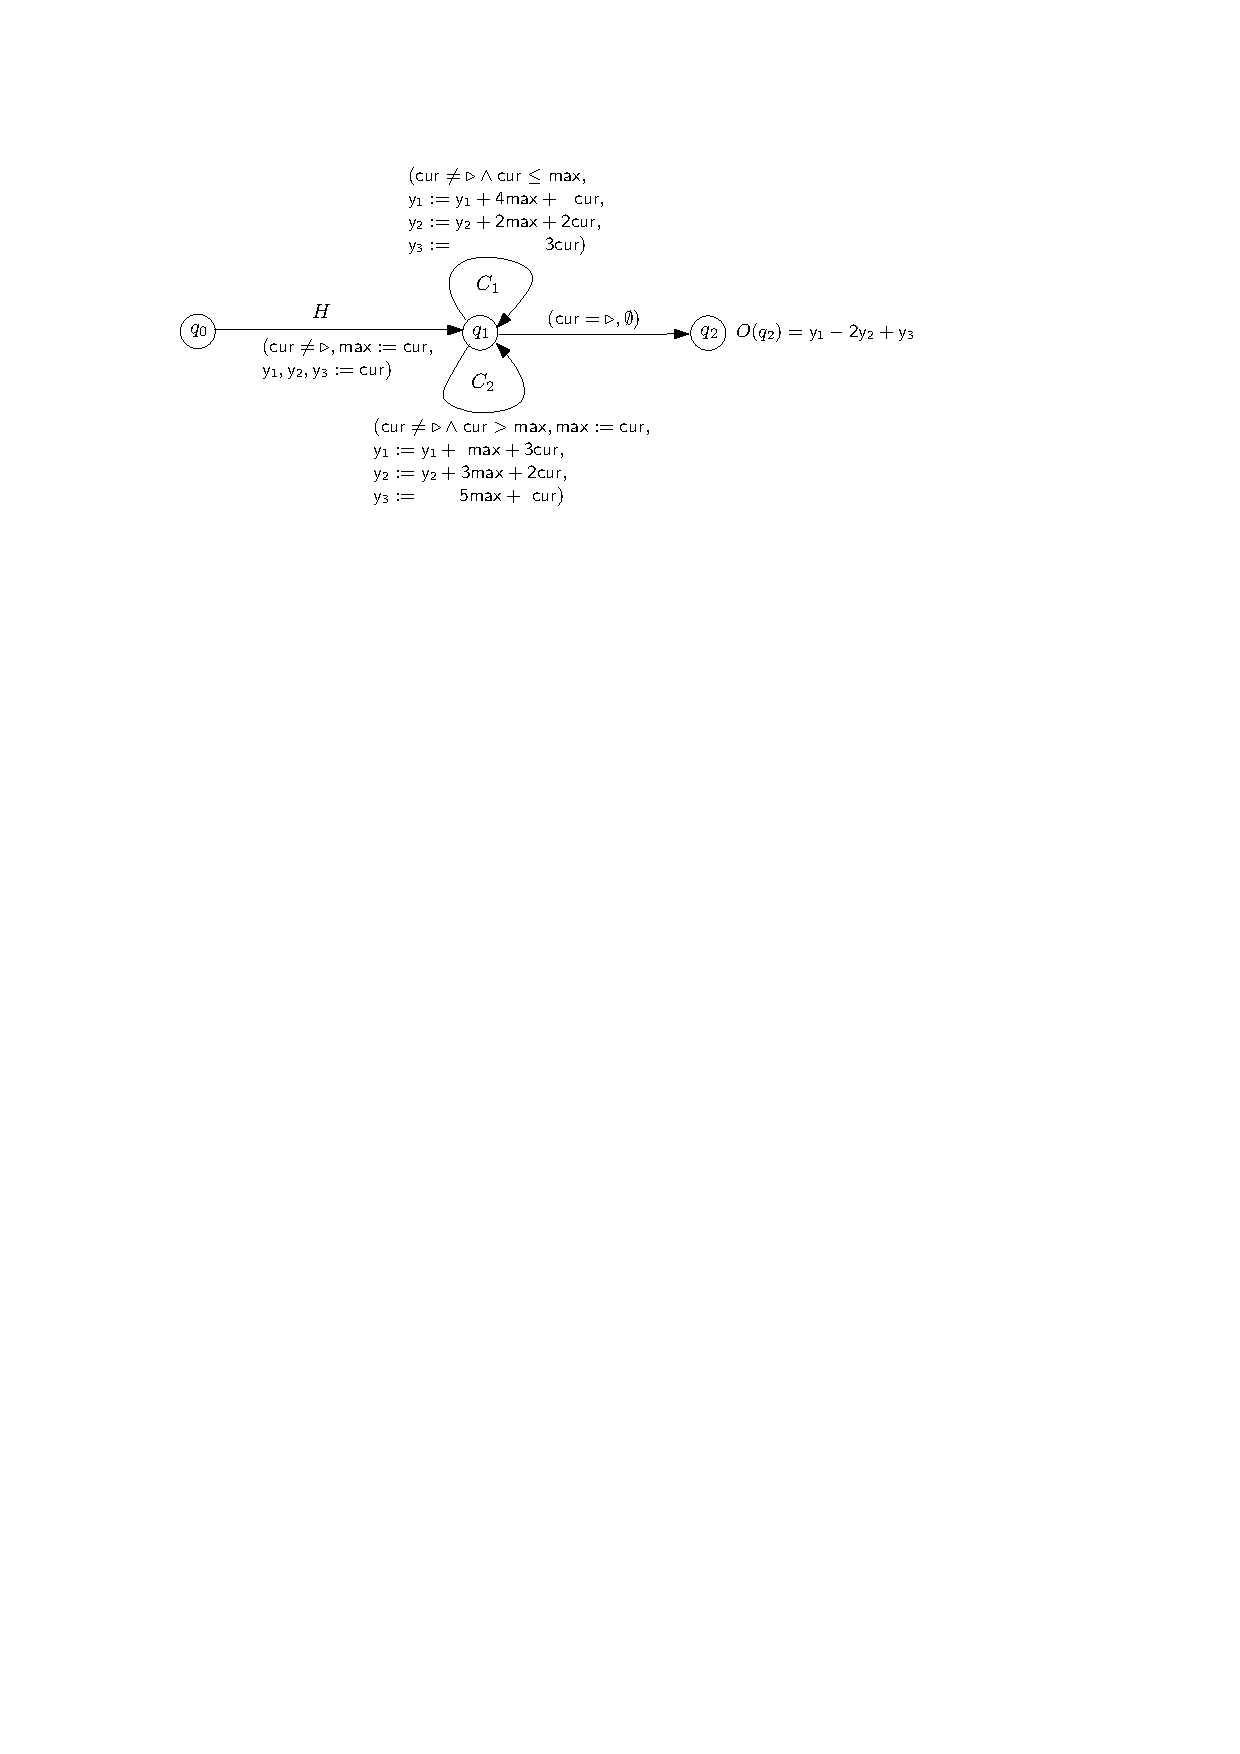
\includegraphics[scale=0.9]{dec-proc-snt-exmp.pdf}
\caption{The SNT $\Ss'_{\max}$: Extending $\Ss_{\max}$ with data variables}\label{fig-dec-proc-snt-exmp}
\end{center}
\end{figure}
%
\end{example}


%!TEX root = main-cav.tex

\vspace{-0.5cm}
\subsection{Decision procedure for generalized lassos}\label{sec-glasso}
\vspace{-1mm}
%
%\yfc{newly added}
In this section, we present a decision procedure for SNTs whose transition graphs are generalized lassos. From Proposition~\ref{prop-sum-cycle}, we know that the coefficients containing the cycle counter variable $\ell$ in $\sumf^{(C^\ell,\initval)}(y_j)$ can be non-zero when $\cstl^{\circled{C}}_{j}=1$. The non-zero coefficients may propagate to the output expression.  In such a case, 
because the SNTs are ``transition-enabled'' (i.e. for any sequence of transitions, a corresponding run exists), %
%if according to the reachability graph, for any $c>0$, there exists a run traversing $C$ more than $c$ times, then 
intuitively, one can pick a run corresponding to a very large $\ell$ so that it dominates the value of the output expression and makes the output non-zero. 
In the decision procedure we are going to present, we first check if the handle of the generalized lasso produces a non-zero output in Step I.
We then check in Step II the coefficients containing $\ell$ in the output expression is non-zero. If this does not happen, then we show in Step III that the non-zero ouput problem of SNT can be reduced to a finite state reachability problem and thus can be easily decided.

Before presenting the decision procedure, we introduce some notations.
Let $e$ be an expression consisting of symbolic values $\initval(z)$ for $z\in X\cup Y$ and variables $\vard_1, \dots, \vard_{s}$ corresponding to the values of the input data word. More specifically, let $e:=\mu_0 + \mu_1 \initval(z_1) +\dots + \mu_{k+l} \initval(z_{k+l}) + \xi_1 \vard_1 + \dots + \xi_{s} \vard_{s}$,
such that $\mu_0,\mu_1,\dots,\mu_{k+l}, \xi_1,\dots,\xi_{s}$ are expressions containing only constants and loop counter variables.
Then we call $\mu_0$ the \emph{constant atom}, $\mu_i \initval(z_i)$ the $\initval(z_i)$-atom for $i\in[k+l]$, and $\xi_j \vard_j$ the $\vard_j$-atom for $j\in[s]$ of the expression $e$. Moreover, $\mu_1, \dots, \mu_{k+l}, \xi_1,\dots, \xi_{s}$ are called the \emph{coefficients} and $\initval(z_1), \dots, \initval(z_{k+l}), \vard_1. \dots, \vard_{s}$ the \emph{subjects} of these atoms.
A non-constant atom is said to be \emph{nontrivial} if its coefficient is \emph{not} identical to zero.

In the rest of this subsection, we assume that the transition graph of $\Ss$ comprises a handle $H=q_0 \xrightarrow{(g_1,\eta_1)} q_1 \dots q_{m-1} \xrightarrow{(g_m,\eta_m)} q_{m}$ and a collection of simple cycles $C_1,\dots,C_n$ such that $q_m$ is the unique state shared by each pair of distinct cycles from $\{C_1,\dots,C_n\}$. Moreover, without loss of generality, we assume that $O(q_m) = a_0 + a_1 x_1 + \dots + a_k x_k + b_1 y_1 + \dots + b_l y_l$, and $O(q)$ is undefined for all the other states $q$.

A \emph{cycle scheme} $\schm$ is a path $C_{i_1}^{\ell_1} C_{i_2}^{\ell_2} \dots C_{i_t}^{\ell_t}$ such that $i_1,\dots,i_t \in [n]$, $\ell_1,\dots, \ell_t \ge 1$, and for each $j\in [t-1]$, $i_j \neq i_{j+1}$. Intuitively, $\schm$ is a path obtained by first iterating $C_{i_1}$ for $\ell_1$ times, then $C_{i_2}$ for $\ell_2$ times, and so on. From Proposition~\ref{prop-sum-cycle} and Corollary~\ref{cor-comp-two-paths}, a symbolic valuation $\sumf^{(\schm,\initval)}$ can be constructed 
to summarize the computation of $\Ss$ on $\schm$. 


\begin{lemma}\label{prop-cycle-schm}
Suppose $\schm=C_{i_1}^{\ell_1} C_{i_2}^{\ell_2} \dots C_{i_t}^{\ell_t}$ is a cycle scheme, and $\initval$ is a symbolic valuation representing the initial values of the control and data variables. 
For all $j' \in  I^{\circled{C_{i_{1}}}}_{pe}$, let $r_{j'}$ be the largest number $r \in [t]$ such that $j'\in\bigcap_{s\in[r]} I^{\circled{C_{i_{s}}}}_{pe}$, i.e., $x_{j'}$ remains persistent when traversing $C_{i_1}^{\ell_1} C_{i_2}^{\ell_2} \dots C_{i_{r_{j'}}}^{\ell_{r_{j'}}}$.
Then for each $j\in [l]$ and $j' \in  I^{\circled{C_{i_{1}}}}_{pe}$, the coefficient of the $\initval(x_{j'})$-atom in $\sumf^{(\schm,\initval)}(y_j)$ is 
\begin{center}
\resizebox{0.8\hsize}{!}{
$e+\sum\limits_{s_1\in[r_{j'}]}  
\left(1+\lambda^{\circled{C_{i_{s_1}}}}_{j} + \dots + (\lambda^{\circled{C_{i_{s_1}}}}_{j})^{\ell_{s_1}-1} \right) \csta^{\circled{C_{i_{s_1}}}}_{j,j'}\prod\limits_{{s_2}\in[{s_1}+1,t]}\left(\lambda^{\circled{C_{i_{s_2}}}}_{j}\right)^{\ell_{s_2}}$},
\end{center}
where (1) $e\!=\!0$ when $r_{j'}\!=\!t$ and (2) $e=(\lambda^{\circled{C_{i_s}}}_{j})^{\ell_s-1} \csta^{\circled{C_{i_{s}}}}_{j,j'} \prod\limits_{{s'}\in[s+1,t]}\left(\lambda^{\circled{C_{i_{s'}}}}_{j}\right)^{\ell_{s'}}$ with $s=r_{j'}+1$ when $r_{j'}<t$.\\
The constant atom of $\sumf^{(\schm,\initval)}(y_j)$ is 
\begin{center}
\resizebox{0.7\hsize}{!}{$
\sum\limits_{{s_1}\in[t]}
\left(1+\lambda^{\circled{C_{i_{s_1}}}}_{j} + \dots + (\lambda^{\circled{C_{i_{s_1}}}}_{j})^{\ell_{s_1}-1} \right)
\cste^{\circled{C_{i_{s_1}}}}_{j} 
\prod\limits_{{s_2}\in[{s_1}+1,t]}\left(\lambda^{\circled{C_{i_{s_2}}}}_{j}\right)^{\ell_{s_2}}$}
\end{center}
Moreover, for all $j\!\in\! [l]$, in $\sumf^{(\schm,\initval)}(y_j)$, only the constant atom and the coefficients of the $\initval(x_{j'})$-atoms with $j' \!\in\!I^{\circled{C_{i_{1}}}}_{pe}$ contain a subexpression of the form $ \mu_\schm \ell_1$ for some~$\mu_\schm\in \intnum$.
\end{lemma}
Notice that above, $\lambda^{\circled{C_{i_{s_1}}}}_j\in\{0,1\}$ for $j\in[l]$ and $s_1\in [t]$. Hence the value of $(1+\lambda^{\circled{C_{i_{s_1}}}}_{j} + \dots + (\lambda^{\circled{C_{i_{s_1}}}}_{j})^{\ell_{s_1}-1} )$ can only be $1$ or $\ell_{s_1}$ and $\left(\lambda^{\circled{C_{i_{s_2}}}}_{j}\right)^{\ell_{s_2}}\in\{0,1\}$.
Therefore, both the constant atom and the coefficient of the $\initval(x_{j'})$-atom with $j'\in I^{\circled{C_{i_{1}}}}_{pe}$ can be rewritten to the form of $c_0+c_1\ell_1+c_2\ell_2+\dots+c_t\ell_t$ for $c_0\ldots c_t\in \intnum$. Note that some of $c_0\ldots c_t$ might be zero.




%We are ready to present the decision procedure. By the ``well-defined'' and ``uniquely-valued'' constraints of normalized SNTs, without loss of generality, we assume that $I^{\circled{H}}_{tr}=[k]$, that is, after traversing $H$, the values of all control variables become defined.
%Under the assumption, 
We are ready to present the decision procedure. At first, we observe that  after traversing $H$ with the initial values of the variables given by $\sval_0$ (recall that $\sval_0$ assigns mutually distinct values to the variables from $X \cup Y$), for each $j' \in I^{\circled{H}}_{tr}$, the value of the control variable $x_{j'}$ becomes $\vard^{\circled{H}}_{\pi^{\circled{H}}(j')}$,  more formally, $\sumf^{(H,\sval_0)}(x_{j'})=\vard^{\circled{H}}_{\pi^{\circled{H}}(j')}$.

In Step I, we check if $\eval{O(q_m)}{\sumf^{(H,\sval_0)}}$ is not identical to zero.
This can be done by checking if the constant-atom or the coefficient of some non-constant atom of the output expression $\eval{O(q_m)}{\sumf^{(H,\sval_0)}}$ is not identical to zero.
%We first find in the reachability graph $G_{\Ss}$ the set of paths $H_{G_{\Ss}}$ corresponding to $H$. Each path in $H_{G_{\Ss}}$ induces an equivalence relation between the subjects of the atoms. 
%For each path $H_{G_{\Ss}}$, we first merge the coefficients of atoms with equivalent subjects. Then we report the output is not identical to zero if the coefficient of some atoms or the constant atom is not zero.
\smallskip\\
\framebox[\textwidth]{
\begin{minipage}{0.95\textwidth}
\noindent {\bf Step I}. Decide whether $\eval{O(q_m)}{\sumf^{(H,\sval_0)}}$ is not identical to zero.
If the answer is yes, then the decision procedure terminates and returns the answer $\ltrue$. Otherwise, go to Step II.
\end{minipage}
}\bigskip

\noindent{\it Complexity analysis of Step I}. Since $\sumf^{(H,\sval_0)}$ can be computed in polynomial time from $H$, it follows that Step I can be done in polynomial time.

\smallskip

The goal of Step II is either showing that in $f=\eval{O(q_m)}{\sumf^{(\schm,\sumf^{(H,\sval_0)})}}$, all subexpressions containing the cycle counter variables are identical to zero and hence can be ignored or showing that $f$ is not identical to zero. Let $\schm=C_{i_1}^{\ell_1} C_{i_2}^{\ell_2} \dots C_{i_t}^{\ell_t}$ be a cycle scheme. From Lemma~\ref{prop-cycle-schm}, for each $j'\in I^{\circled{C_{i_1}}}_{pe}$ and symbolic valuation $\sval$, the only subexpression containing $\ell_1$ in the coefficient of $\initval(x_{j'})$-atom of $\eval{O(q_m)}{\sumf^{(\schm,\initval)}}$ is
\begin{center}
	\resizebox{0.7\hsize}{!}{$
\sum \limits_{1 \le j \le l} 
b_j \left((\cstl^{\circled{C_{i_2}}}_{j})^{\ell_2} \dots (\cstl^{\circled{C_{i_t}}}_{j})^{\ell_t}\right) 
\left(1+\cstl^{\circled{C_{i_1}}}_{j} + \dots + (\cstl^{\circled{C_{i_1}}}_{j})^{\ell_1-1} \right) \csta^{\circled{C_{i_1}}}_{j,j'}.
\hspace{4mm} (\ast)
$}
\end{center}
Since $\cstl^{\circled{C_{i_1}}}_{j}, \cstl^{\circled{C_{i_2}}}_{j}, \dots, \cstl^{\circled{C_{i_t}}}_{j} \in \{0, 1\}$, the expression $(\ast)$  can be rewritten as  
 $\mu_{\schm, (i_1,j')} \ell_1 + \nu_{\schm, (i_1,j')}$ for some integer constants $\mu_{\schm, (i_1,j')}$ and $\nu_{\schm, (i_1,j')}$. 
 
The only subexpression containing $\ell_1$ in the constant atom of  $\eval{O(q_m)}{\sumf^{(\schm,\initval)}}$ is
\begin{center}
	\resizebox{0.7\hsize}{!}{$
\sum \limits_{1 \le j \le l} b_j
\begin{array}{l}
 \left((\lambda^{\circled{C_{i_2}}}_{j})^{\ell_2} \dots (\lambda^{\circled{C_{i_t}}}_{j})^{\ell_t}\right)
\left(1+\lambda^{\circled{C_{i_1}}}_{j} + \dots + (\lambda^{\circled{C_{i_1}}}_{j})^{\ell_1-1} \right) \cste^{\circled{C_{i_1}}}_{j}. \hspace{2mm} (\ast\ast)
\end{array}
$}
\end{center}
%
The expression $(\ast\ast)$ can be rewritten as $\mu_{\schm,(i_1,0)} \ell_1 + \nu_{\schm,(i_1,0)}$ for some integer constants $\mu_{\schm, (i_1,0)}$ and $\nu_{\schm, (i_1,0)}$. If $\mu_{\schm,(i_1,0)}=0$ and $\mu_{\schm,(i_1,j')}=0$ for all $j' \in I^{\circled{C_{i_1}}}_{pe}$, then we can ignore all subexpressions containing the cycle counter variable $\ell_1$ in   $\eval{O(q_m)}{\sumf^{(\schm,\initval)}}$, i.e., the subexpressions $\mu_{\schm,(i_1,0)}\ell_1$ and $\mu_{\schm,(i_1,j')}\ell_1$ for all $j' \in I^{\circled{C_{i_1}}}_{pe}$.\smallskip\\
\framebox[\textwidth]{
	\begin{minipage}{0.95\textwidth}
		\noindent {\bf Step II}. For each $i_1 \in [n]$, check all cycle scheme $\schm=C_{i_1}^{\ell_1} C_{i_2} \dots C_{i_t}$ such that $i_2,\dots,i_t$ are mutually distinct. There are only finitely many this kind of cycle schemes. If 
		one of the following constraints is satisfied, then return $\ltrue$. \\(1) There is $j' \in  I^{\circled{C_{i_1}}}_{pe}$ such that $\mu_{\schm,(i_1,j')} \neq 0$. (2) $\mu_{\schm,(i_1,0)} \neq 0$.
		%
		If the decision procedure has not returned yet, then go to Step III.
	\end{minipage}
}\bigskip

\noindent{\it Complexity analysis of Step II}. Since $i_1,\dots, i_t$ are mutually distinct, the number of cycle schemes $\schm = C_{i_1}^{\ell_1} C_{i_2} \dots C_{i_t}$ in Step II is exponential over the number of cycles in the generalized lasso. Once the cycle scheme is fixed, the two constraints in Step II can be decided in polynomial time. Therefore, the complexity of Step II is exponential over the number of cycles in the generalized lasso.

\smallskip

If there exists $j' \in I^{\circled{C_{i_1}}}_{pe}$ such that $\mu_{\schm,(i_1,j')} \neq 0$, then we let $\vard^{\circled{H}}_{\pi^{\circled{H}}(j')} \neq 0$ and $\ell_1$ be arbitrarily large, so that the coefficient of the  $\vard^{\circled{H}}_{\pi^{\circled{H}}(j')}$-atom in $\eval{O(q_m)}{\sumf^{(\schm,\sumf^{(H,\sval_\bot)})}}$, which includes the expression $\mu_{\schm, (i_1,j')} \ell_1 + \nu_{\schm, (i_1,j')}$, dominates $\eval{O(q_m)}{\sumf^{(\schm,\sumf^{(H,\sval_\bot)})}}$. This is sufficient to make $\eval{O(q_m)}{\sumf^{(\schm,\sumf^{(H,\sval_\bot)})}}$ non-zero. Similarly, if $\mu_{\schm,(i_1,0)} \neq 0$, then we can let $\ell_1$ arbitrarily large to make the expression $\eval{O(q_m)}{\sumf^{(\schm,\sumf^{(H,\sval_\bot)})}}$ non-zero.
Similar arguments can be applied for $\ell_2\dots\ell_n$.

If Step II does not return $\ltrue$, we show below that for all cycle schemes $\schm_1=C_{i_1}^{\ell_1} C_{i_2}^{\ell_2} \dots C_{i_{s_1}}^{\ell_{s_1}}$ with $i_1,i_2,\dots,i_{s_1} \in [n]$, all subexpressions containing cycle counter variables in $\eval{O(q_m)}{\sumf^{(\schm,\initval)}}$ are identical to zero and hence can be removed. Let ${i'_2} \dots {i'_{s_2}}$ be the sequence obtained from $i_2 \dots i_{s,1}$ by keeping just one copy for each duplicated index therein.  
In Step II we already checked a cycle scheme $\schm_2=C_{i_1}^{\ell_1} C_{i'_2} \dots C_{i'_{s_2}}$. Step II guarantees that all subexpressions containing $\ell_1$ in 
$\eval{O(q_m)}{\sumf^{(\schm_2,\initval)}}$ are identical to zero and hence can be removed.
Because for all $j\in[l]$, $\cstl^{^{\circled{C_1}}}_j, \dots, \cstl^{^{\circled{C_n}}}_j \in \{0,1\}$,   $(\lambda^{\circled{C_{i_2}}}_{j})^{\ell_2} \dots (\lambda^{\circled{C_{i_{s_1}}}}_{j})^{\ell_{s_1}} = \lambda^{\circled{C_{i'_2}}}_{j} \dots \lambda^{\circled{C_{i'_{s_2}}}}_{j}$. We proved that the $(\ast)$ and $(\ast\ast)$ style expressions are equivalent in both $\schm_1$ and $\schm_2$.
Hence we can also remove all subexpressions containing $\ell_1$ from  $\eval{O(q_m)}{\sumf^{(\schm_1,\initval)}}$, without affecting its value.
Those subexpressions containing $\ell_2$ can also be removed by considering the cycle scheme $\schm_3=C_{i_2}^{\ell_2} C_{i''_3} \dots C_{i''_{s_3}}$ and applying a similar reasoning, where the sequence ${i''_3} \dots {i''_{s_3}}$ is obtained from ${i_3} \dots  i_{s_1}$, similarly to the construction of ${i'_2} \dots {i'_{s_2}}$ from $i_2 \dots i_{s,1}$. The same applies to all other cycle counter variables $\ell_3,\dots,\ell_{s_1}$.
We use the notation ${\sumf^{(\schm,\initval)}}^-(y_j)$ to denote the expression obtained by removing from the constant atom and coefficients of the non-constant atoms of $\sumf^{(\schm,\initval)}(y_j)$ all subexpressions containing cycle counter variables, for all $y_j \in Y$. 

\begin{lemma}\label{prop-bnd-domain-1}
	Suppose that the decision procedure has not returned $\ltrue$ after Step~II. For each cycle scheme $\schm$, let $f=\eval{O(q_m)}{\sumf^{(\schm, \sumf^{(H,\sval_\bot)})}}$ and $f'=\eval{O(q_m)}{{\sumf^{(\schm, \sumf^{(H,\sval_\bot)})}}^-}$. For all valuation $\rho$, $\eval{f}{\rho}\neq 0$ iff $\eval{f'}{\rho} \neq 0$.
\end{lemma}





\begin{lemma}\label{prop-bnd-domain-2}
Suppose that the decision procedure has not returned yet after Step II. 
For all cycle scheme $\schm$ and $y_j \in Y$, the constant atom and the coefficients of all non-constant atoms in ${\sumf^{(\schm, \sumf^{(H,\initval_\bot)})}}^-(y_j)$ are from a finite set $U \subset \intnum$ comprising \\ (1)
the constant atom and the coefficients of the non-constant atoms in the expression ${\sumf^{(C^{\ell_i}_{i}, \sumf^{(H,\initval_\bot)})}}^-(y_j)$ for $i\in [n]$ and $\ell_i \in \{1,2\}$,\smallskip\\(2) the numbers $\csta^{\circled{C_{s_2}}}_{j,j'} + \cstb^{\circled{C_{s_1}}}_{j,\pi^{\circled{C_{s_1}}}(j')}$ and $\csta^{\circled{C_{s_1}}}_{j, j''} + \csta^{\circled{C_{s_2}}}_{j,j''}$, where  $s_1,s_2 \in [n], j\in[l],j' \in I^{\circled{C_{s_1}}}_{tr} \cap I^{\circled{C_{s_2}}}_{tr},  j'' \in [k]$. 

\end{lemma}

For each cycle scheme $\schm$, an abstraction of ${\sumf^{(\schm, \sumf^{(H,\initval_\bot)})}}^-$, denoted by $\abs(\schm)$,  is the union of the following three sets:
(1)~constant atom: $\{(0, ( {\cste^{(\schm)}_{1}}^-,\dots, {\cste^{(\schm)}_l}^-))\}$. 
(2)~control variable atom: $\{(j', (c_{j',1},\dots, c_{j', l})) \mid j' \in [k]\}$, where $c_{j', j}$ is the coefficient of the ${\sumf^{(\schm,\sumf^{(H,\sval_\bot)})}}^-(x_{j'})$-atom in ${\sumf^{(\schm,\sumf^{(H,\sval_\bot)})}}^-(y_{j})$ for $j\in[l]$. (3)~data variable atom: $\{(k+1, (c_1,\dots,c_l))\}$, where $(c_1,\dots,c_l) \in U^l$ is the coefficients of the $\vard'$-atom in ${(\sumf^{(\schm,\sumf^{(H,\sval_\bot)})}}^-(y_{j})$ for all $j \in [l]$ and $\vard'\not\in \{{\sumf^{(\schm,\sumf^{(H,\sval_\bot)})}}^-(x_{j'})\mid x_{j'}\in X\}$.
Let $\mathscr{A}=\bigcup \{\abs(\schm) \mid \schm \mbox{ a cycle scheme}\}$. Then $\mathscr{A}$ can be constructed as follows. We first compute $\abs(HC_1), \ldots \abs(HC_n)$ and then compute the next abstract elements from them w.r.t. $C_1\ldots C_n$ until reached a fixed point.\medskip\\
\framebox[\textwidth]{
	\begin{minipage}{0.95\textwidth}
		\noindent {\bf Step III} We first construct the set $\mathscr{A}$ and then. 
		\begin{enumerate}
			\item Check whether there is $(0,(c_{0,1},\dots,c_{0,l})) \in \mathscr{A}$ such that $a_0+b_1 c_{0,1}+\dots + b_l c_{0,l} \neq 0$. If the answer is yes, then return $\ltrue$.
			%
			\item Check whether there are $j' \in [k]$ and $(j', (c_{j',1},\dots,c_{j',l})) \in \mathscr{A}$ such that $a_{j'} + b_1 c_{j',1} + \dots + b_l c_{j',l} \neq 0$. If the answer is yes, then return $\ltrue$. 
			%
			\item Check whether there is $(k+1,(c_1,\dots,c_l)) \in \mathscr{A}$ such that $b_1 c_1 + \dots + b_l c_l \neq 0$. If the answer is yes, then return $\ltrue$. 
		\end{enumerate}
		If the decision procedure has not returned yet, return $\lfalse$.
	\end{minipage}
}\smallskip\\

\noindent {\it Complexity analysis of Step III}. The size of the set $U$ is polynomial over the size of the generalized lasso (i.e. the size of the transitions in the generalized lasso). The size of $\mathscr{A}$ is exponential over $l$, the number of data variables. The three conditions in Step III can be checked in time polynomial over the size of $\mathscr{A}$. In summary, the complexity of Step III is exponential over the number of data variables.


\vspace{-2mm}
\subsection{Decision procedure for SNTs}\label{sec-gflat}
\vspace{-1mm}

We generalize the decision procedure for the case that the transition graphs of the SNTs are generalized lassos to the full class of SNTs.
We first define a \emph{generalized multi-lasso} as a sequence $\gmlasso= H_1 (C_{1,1},\dots,C_{1,n_1}) H_2 (C_{2,1},\dots,C_{2,n_2}) \dots H_r (C_{r,1},\dots, C_{r, n_r})$ s.t. (1) for each $s\in[r]$, $H_s=q_{s,1} \xrightarrow{(g_2,\eta_2)} q_{s,2} \dots q_{s,m_s-1} \xrightarrow{(g_{m_s},\eta_{m_s})} q_{s,m_s}$ is a generalized lasso, (2) for $1 \leq s< s' \leq r$, $H_s (C_{s,1},\dots,C_{s, n_s})$ and $H_{s'} (C_{s', 1},\dots,C_{s', n_{s'}})$ are state-disjoint, except the case that when $s'=s+1$, $q_{s, m_s}=q_{s',1}$, and (3) $q_{1,1}=q_0$.

Since the transition graph of $\Ss$ can be seen as a finite collection of generalized multi-lassos, in the following, we shall present the decision procedure by showing how to decide the non-zero output problem for generalized multi-lassos. 

We fix a generalized multi-lasso below and assume without loss of generality that $O(q_{r,m_r})=a_0+a_1 x_1 + \dots + a_k x_k + b_1 y_1  + \dots + b_l y_l$ and $O(q')$ is undefined for every other state $q'$ in $\gmlasso$.

\smallskip
\hspace{8mm} $\gmlasso= H_1 (C_{1,1},\dots,C_{1,n_1}) H_2 (C_{2,1},\dots,C_{2,n_2}) \dots H_r (C_{r,1},\dots, C_{r, n_r})$.

\subsubsection{Step I':} We do the same analysis as in Step I for the path $H_1\dots H_r$.
\hide{\smallskip\\
\framebox[\textwidth]{
	\begin{minipage}{0.95\textwidth}
		\noindent {\bf Step I$'$}. We do the same analysis as in Step I for the path $H_1\dots H_r$.
	\end{minipage}
}\smallskip}
\subsubsection{Step II':}
Let $s\in [1,r-1]$. In order to analyze the set of cycles $\Cc=\{C_{s,1},\dots,C_{s,n_{s}}\}$, next we show how to summarize effect of the path $H_{s+1}\dots H_r$ to $O(q_{s, m_{s}})$, which is shared by all those cycles in $\Cc$.
Suppose that $\eval{O(q_{r,m_r})}{\sumf^{(H_{s+1}\dots H_{r}, \initval)}}=a_0+a_1 \initval(x_1)+ \dots + a_k \initval(x_k) + b_1 \initval(y_1) + \dots + b_l \initval(y_l)+e$, where $e$ is a linear combination of the data variables that represent the data values introduced when traversing $H_{s+1}\dots H_r$. Since we already passed Step I, we know that $e$ should be identical to zero. 
%the constant atom is $a_{s,0}$, the coefficient of the $\initval(x_j)$-atom is $a_{s, j}$ for each $j \in [k]$, and the coefficient of the $\initval(y_{j'})$-atom is $b_{s, j'}$ for each $j' \in [l]$. 
Moreover, we know that $\initval(x_1)\dots\initval(x_k)$ and $\initval(y_1)\ldots \initval(y_l)$ are values of $x_1\dots x_k$ and $y_1 \dots y_l$ at the state $q_{s, m_{s}}$. Therefore, we can summarize the effect of $H_{s+1}\dots H_{r}$ to $q_{s, m_{s}}$ by letting
$O(q_{s, m_{s}}):=a_0+a_1 x_1 + \dots + a_k x_k + b_1 y_1 + \dots + b_l y_l$ and $O(q')$ is undefined for every other state $q'$.\smallskip\\
\framebox[\textwidth]{
	\begin{minipage}{0.95\textwidth}
\noindent {\bf Step II$'$}.  For each $s\in [r]$ and $s'\in [n_s]$, we check each cycle scheme $\schm = C^{\ell_1}_{s,s'} C_{i_{2}} \dots C_{i_{t}}$ such that $C_{i_{2}} \dots C_{i_{t}}\in \{C_{s, 1}, \dots, C_{s,n_s},\dots, C_{r,1}, \dots, C_{r,n_r}\}$ and $C_{i_{2}} \dots C_{i_{t}}$ are mutually distinct by performing an analysis of the expression $\eval{ O(q_{s, m_{s}})} {\sumf^{(\schm,\sumf^{(H_1 \dots H_{s}, \initval)} ) } }$, in a way similar to Step II. If the decision procedure does not return during the analysis, then go to Step III$'$.
	\end{minipage}
}\bigskip\\
Intuitively, in Step II$'$, during the analysis of $\eval{ O(q_{s, m_{s}})} {\sumf^{(\schm,\sumf^{(H_1 \dots H_{s}, \initval)} ) } }$, the effect of the paths $H_{s+1},  \dots,  H_r$ and the cycles $C_{i_{2}}, \dots, C_{i_{t}}$ to the atom coefficients containing cycle counter variables are expressions of the form $\cstl^{\circled{H_{s+1}}}_j \dots \cstl^{\circled{H_{r}}}_j  \cstl^{\circled{C_{i_{2}}}}_j \dots \cstl^{\circled{C_{i_{t}}}}_j $ for $j \in [l]$. Since $O(q_{s, m_{s}})$ has already taken into consideration the expressions $\cstl^{\circled{H_{s+1}}}_j \dots \cstl^{\circled{H_{r}}}_j$ for $j \in [l]$. In Step II$'$, we can do the analysis as if we have a generalized lasso where the handle is $H_1\dots H_s$ and the collection of cycles is $\{C_{s,1},\dots, C_{s,n_s}$, $\dots$, $C_{r,1},\dots, C_{r,n_r}\}$. 
%$\schm=C^{\ell_{s, 1}}_{i_{s,1}} \dots C^{\ell_{s, t_s}}_{i_{s, t_s}} C^{\ell_{s+1, 1}}_{i_{s+1, 1} } \dots C^{\ell_{s+1, t_{s+1}}}_{i_{s+1, t_{s+1}} } \dots C^{\ell_{r, 1}}_{i_{r,1}} \dots C^{\ell_{r, t_r}}_{i_{r, t_r}} $, where for each $s': s \le s' \le r$, $i_{s',1},\dots, i_{s', t_{s'}} \in [n_{s'}]$, 
%%%%%%%%%%%%%%%%%%%%%%%%%%%%%%%%%%%%%%%%%%%%%%%%%%%
%%%%%%%%%%%%%%%%%%%%%%%%%%%%%%%%%%%%%%%%%%%%%%%%%%%
%%%%%%%%%%%%%%%%%%%%%%%%%%%%%%%%%%%%%%%%%%%%%%%%%%%
\hide
{
At first, by using $O(q_m)$, we do the following computation, similarly to Step II: For each $i_1: 1 \le i_1 \le n$, if there are a cycle scheme $\schm$  
$HC_{i_1}^{\ell_1} C_{i_2}^{\ell_2} \dots C_{i_t}^{\ell_t}
$
or 
$HC_{i_1}^{\ell_1} C_{i_2}^{\ell_2} \dots C_{i_t}^{\ell_t} (C'_{i'_1})^{\ell'_1} (C'_{i'_2})^{\ell'_2} \dots (C'_{i'_{t'}})^{\ell'_{t'}}$,
and $j' \le k$ such that 
\begin{itemize}
\item $i_2,\dots,i_t \le n$ are mutually distinct, $\ell_2 = \dots = \ell_t = 1$, 
%
\item $i'_1,\dots,i'_{t'} \le n'$ are mutually distinct, $\ell'_2 = \dots = \ell'_{t'} = 1$, 
%
\item $\pi_{C_{i_1}}(j')=j'$, and $\mu_{\schm,(i_1,j')} \neq 0$ (recall that $\mu_{\schm,(i_1,j')}$ is obtained from the coefficient of $d^{(0)}_{\pi_H(j')-k}$ in  $\chi_\schm(O(q_m))$), 
\end{itemize}
then return $\ltrue$. 

Then by using $O(q'_{m'})$, we do the following: For each $i'_1: 1 \le i'_1 \le n'$, if there are a cycle scheme $\schm' =(C'_{i'_1})^{\ell'_1} (C'_{i'_2})^{\ell'_2} \dots (C'_{i'_{t'}})^{\ell'_{t'}}$, and $j' \le k$ such that
\begin{itemize}
\item $i'_2,\dots,i'_t \le n'$ are mutually distinct, $\ell'_2 = \dots = \ell'_t = 1$, 
%
\item $\pi_{C'_{i_1}}(j')=j'$, and $\mu_{\schm',(i'_1,j')} \neq 0$ (here $\mu_{\schm',(i_1,j')}$ is obtained from the coefficient of $d''_{j'}$ in  $\chi_{\schm'}(O(q'_{m'}))$, where $d''_1,\dots,d''_k$ denote the initial data values of $x_1,\dots,x_k$ respectively),
\end{itemize}
then return $\ltrue$. 

Similarly, we can apply an analysis for the constant coefficient to $\chi_\schm(O(q_m))$. 


If the decision procedure has not return yet, then go to Step III$'$. \qed
}
%%%%%%%%%%%%%%%%%%%%%%%%%%%%%%%%%%%%%%%%%%%%%%%%%%%
%%%%%%%%%%%%%%%%%%%%%%%%%%%%%%%%%%%%%%%%%%%%%%%%%%%
%%%%%%%%%%%%%%%%%%%%%%%%%%%%%%%%%%%%%%%%%%%%%%%%%%%
\subsubsection{Step III':}
After Step II$'$, if the decision procedure has not returned yet, then similar to Lemma~\ref{prop-bnd-domain-2}, the following hold.
\begin{itemize}
\item For each $s \in [r]$ and each path $\schm=H_1 \schm_1 H_2 \dots H_s \schm_s$ such that for each $s'\in [s]$, $\schm_{s'}$ is a cycle scheme over the collection of cycles $\{C_{s',1},\dots,C_{s',n_{s'}}\}$, it holds that the constant atom and all the coefficients of the non-constant atoms in ${\sumf^{(\schm,\sval_\bot)}}^-(y_j)$ are from a bounded domain $U$.
%
\item Moreover,  an abstraction of $\schm$, denoted by $\abs(\schm)$, can be defined, so that $\mathscr{A}$, which contains the set of $\abs(\schm)$ for the paths $\schm=H_1 \schm_1 H_2 \dots H_s \schm_s$ (where $s \in [r]$), can be computed effectively from 
$H_1, C_{1,1}, \dots, C_{1,n_1},H_2,\dots, H_r,C_{r,1},\dots, C_{r,n_r}$.
\end{itemize}
%Similarly to the generalized lassos, we can construct a finite state automaton $\Aa'$ from $\chi_H,\chi_{C_1},\dots,\chi_{C_n},\chi_{H'}, \chi_{C'_1},\dots,\chi_{C'_{n'}}$ to record the coefficients in the states and simulate the evolvement of these coefficients. The final states of $\Aa$ represent the coefficients obtained when reaching the state $q'_{m'}$ in $\Ss$. 
\framebox[\textwidth]{
	\begin{minipage}{0.95\textwidth}
\noindent {\bf Step III$'$}. We apply the same analysis to $\mathscr{A}$ as in Step III. If the procedure does not return during the analysis, return $\lfalse$.
	\end{minipage}
}\bigskip

\noindent {\it Complexity analysis of Step I$'$-III$'$}. The complexity of Step I$'$ is polynomial over the the maximum length of generalized multi-lassos in $\Ss$. The complexity of Step II$''$ is exponential over the maximum number of simple cycles in generalized multi-lassos. The complexity of Step III$'$ is still exponential over the number of data variables in $\Ss$.

